\documentclass[11pt]{scrartcl}

\usepackage[top=1.5cm]{geometry}
\usepackage{url}
\usepackage{float}
\usepackage{listings}
\usepackage{xcolor}
\usepackage{graphicx}
\usepackage{booktabs}

\setlength{\parindent}{0em}
\setlength{\parskip}{0.5em}

\newcommand{\youranswerhere}{[Your answer goes here \ldots]}
\renewcommand{\thesubsection}{\arabic{subsection}}

\lstdefinestyle{dmrsql}{
  language=SQL,
  basicstyle=\small\ttfamily,
  keywordstyle=\color{magenta!75!black},
  stringstyle=\color{green!50!black},
  showspaces=false,
  showstringspaces=false,
  commentstyle=\color{gray}}

\lstdefinestyle{dmrJava}{
  language=JAVA,
  basicstyle=\small\ttfamily,
  keywordstyle=\color{magenta!75!black},
  stringstyle=\color{green!50!black},
  showspaces=false,
  showstringspaces=false,
  commentstyle=\color{gray}}

\title{
  \textbf{\large Projektaufgabe 3 } \\
  Phase 2 – Implementierung des XPath Accelerators (5 P) \\
  {\large Datenmanagement jenseits von Relationen}
}

\author{
  Gruppen Nummer (e.g. A1, B5, B3) \\
  \large Lastname1 Firstname1, StudentID1 \\
  \large Lastname2 Firstname2, StudentID2 
  \large Sadykova Nargiz, 12129337
}

\begin{document}

\maketitle\thispagestyle{empty}

Dieses Reporting Template dient der Vorbereitung der Abgabe von Phase 2.

\subsection*{Verwendung der Daten aus der DBLP (1 Punkt)}

Geben Sie die folgende Kennzahl bezogen auf \texttt{my\_small\_bib.xml} an:

\begin{itemize}
	\item Anzahl Publikationen von 'Nikolaus Augsten'\footnote{Korrektheit und Vollständigkeit können Sie unter https://dblp.org/pid/76/3961.html überprüfen.}
		\begin{itemize}
		\item ICDE: TODO
		\item VLDB: TODO
		\item SIGMOD: TODO
	\end{itemize}
	\item Position (Zeilennummer von, bis) der Publikationen des Toy-Beispiels in \texttt{my\_small\_bib.xml}
	
	\begin{itemize}
		\item SchmittKAMM23: TODO Lines
		\item HutterAK0L22: TODO Lines
		\item SchalerHS23: TODO Lines
	\end{itemize}
	\item Größe der Datei \texttt{my\_small\_bib.xml} in kB und Zeilenanzahl: TODO
\end{itemize}



\subsection*{Schemaerstellung (1 Punkt).}
Geben Sie die Create Table statements aller von Ihnen angelegten Tabellen an:
\begin{lstlisting}[style=dmrsql]
postgres=# CREATE TABLE accel (
  pre    INTEGER,
  post   INTEGER,
  parent INTEGER,
  kind   TEXT,
  name   TEXT
);

CREATE TABLE content (
  pre  INTEGER,
  text TEXT
);
CREATE TABLE
CREATE TABLE
postgres=# CREATE TABLE attribute ( pre  INTEGER,
  text TEXT
);
\end{lstlisting}

\subsection*{Pre-/Post-Order Annotation (1 Punkt).}
Definieren Sie sich einen \textit{Ausschnitt} aus \texttt{toy\_example.txt}. Berechnen Sie hierfür händisch die Pre-/Post-Order Annotation. Inkludieren Sie diese als Foto / Screenshot oder ähnliches in dieses Dokument. Zeigen Sie dann, dass Ihre Lösung hierfür dieselben Ergebnisse liefert. Sie können Die Mittels Foto / Screenshot belegen oder in der Übung zeigen.

Ausschnitt aus toy_example.txt:
<bib>
	<article mdate="2024-02-05" key="journals/pvldb/SchmittKAMM23">
		<author orcid="0009-0005-7656-7526">Daniel Ulrich Schmitt</author>
		<author>Daniel Kocher</author>
		<author orcid="0000-0002-3036-6201">Nikolaus Augsten</author>
		<author>Willi Mann</author>
		<author>Alexander Miller</author>
		<title>A Two-Level Signature Scheme for Stable Set Similarity Joins.</title>
		<pages>2686-2698</pages>
		<year>2023</year>
		<volume>16</volume>
		<journal>Proc. VLDB Endow.</journal>
		<number>11</number>
		<ee type="oa">https://www.vldb.org/pvldb/vol16/p2686-schmitt.pdf</ee>
		<ee>https://doi.org/10.14778/3611479.3611480</ee>
		<url>db/journals/pvldb/pvldb16.html#SchmittKAMM23</url>
	</article>
	
\begin{figure}[H]
  \centering
  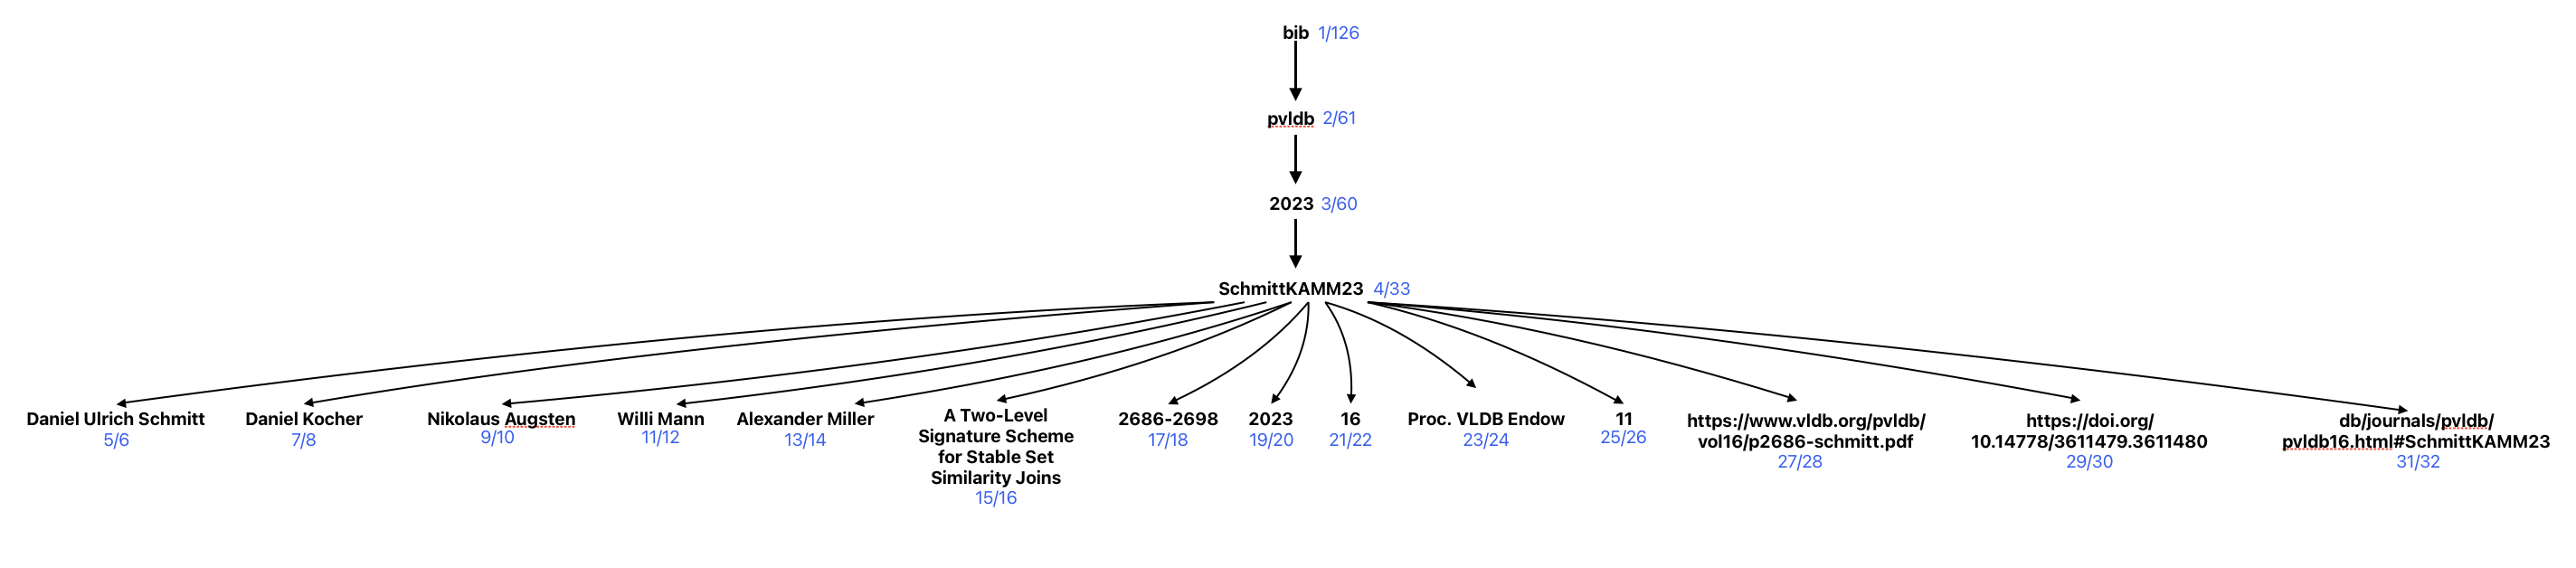
\includegraphics[width=0.8\textwidth]{annotatedtree.png}
\end{figure}

\subsection*{Achse als Fenster (2 Punkt)}
Zeigen Sie, dass die Berechnung der Achsen für die Beispiele aus Phase 1 hier die gleichen Ergebnisse erzeugen:

\begin{table}[h]
	\centering
		\begin{center}
			\begin{tabular}{ l | c c }
				\toprule
				Achse & Ergebnisknoten ID's & Ergebnisgröße\\
				\midrule
				ancestor & ... & ... \\ 
				descendants & ... & ... \\  
				following SchmittKAMM23& ... & ... \\  
				preceeding SchmittKAMM23 & ... & ... \\ 
				following SchalerHS23& ... & ... \\  
				preceeding SchalerHS23& ... & ... \\ 
				\bottomrule
			\end{tabular}
			\end{center}
	\caption{Ergebnisse der XPath-Berechnung auf Edge Modell aus Phase 1}
	\label{tab:ErgebnisseDerXPathBerechnug}
\end{table}

\begin{table}[h]
	\centering
		\begin{center}
			\begin{tabular}{ l | c c }
				\toprule
				Achse & Ergebnisknoten ID's & Ergebnisgröße\\
				\midrule
				ancestor & ... & ... \\ 
				descendants & ... & ... \\  
				following SchmittKAMM23& ... & ... \\  
				preceeding SchmittKAMM23 & ... & ... \\ 
				following SchalerHS23& ... & ... \\  
				preceeding SchalerHS23& ... & ... \\ 
				\bottomrule
			\end{tabular}
			\end{center}
	\caption{Ergebnisse der XPath-Berechnung des XPath-Accelerators aus Phase 2}
	\label{tab:ErgebnisseDerXPathBerechnug}
\end{table}

\subsection*{Zeitmamagement}

Benötigte Zeit pro Person (nur Phase 2): \textbf{Sadykova Nargiz: 4.5 Std.}


\end{document}
